\documentclass[xcolor=dvipsnames,table]{beamer}

\usepackage{latexsym}
\usepackage[utf8]{inputenc}
\usepackage[brazil]{babel}
\usepackage{amssymb}
\usepackage{amsmath}
\usepackage{stmaryrd}
\usepackage{fancybox}
\usepackage{datetime}
\usepackage[T1]{fontenc}
\usepackage{graphicx}
\usepackage{graphics}
\usepackage{url}
\usepackage{algorithmic}
\usepackage{algorithm}
\usepackage{acronym}
\usepackage{array}
\usepackage[normalem]{ulem}

\newtheorem{definicao}{Definio}
\newcommand{\tab}{\hspace*{2em}}

\mode<presentation>
{
  \definecolor{colortexto}{RGB}{0,0,0}
 
  \setbeamertemplate{background canvas}[vertical shading][ bottom=white!10,top=white!10]
  \setbeamercolor{normal text}{fg=colortexto} 

  \usetheme{Warsaw}
}

\title{Máquina de Turing} 

\author{
  Esdras Lins Bispo Jr. \\ \url{bispojr@ufg.br}
  } 
 \institute{
  Teoria da Computação \\Bacharelado em Ciência da Computação}
\date{\textbf{16 de maio de 2016} }

\logo{
\includegraphics[width=1cm]{images/ufgJataiLogo.png}}

\begin{document}

	\begin{frame}
		\titlepage
	\end{frame}

	\AtBeginSection{
		\begin{frame}{Sumário}%[allowframebreaks]{Sumário}
    		\tableofcontents[currentsection]
    		%\tableofcontents[currentsection, hideothersubsections]
		\end{frame}
	}

	\begin{frame}{Plano de Aula}
		\tableofcontents
		%\tableofcontents[hideallsubsections]
	\end{frame}
    
    \section{Pensamento}
	\begin{frame}{Pensamento}
  		\begin{center}
    		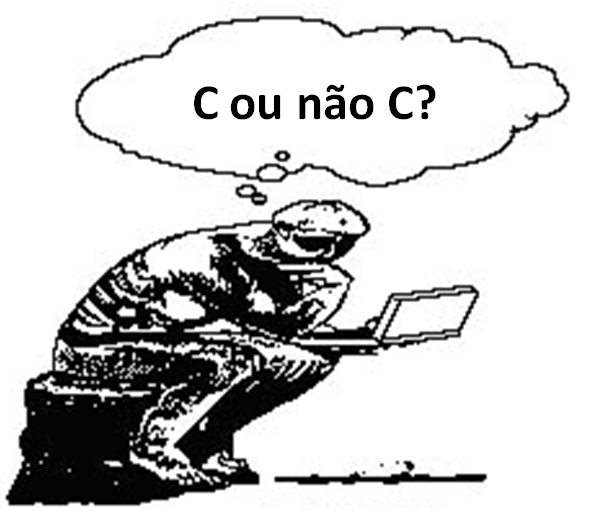
\includegraphics[width=7cm]{images/pensamento.png}
  		\end{center}
	\end{frame}
	
\begin{frame}{Pensamento}
		\begin{columns}
			\column{.4\textwidth}  		
		  		\begin{center}
		    		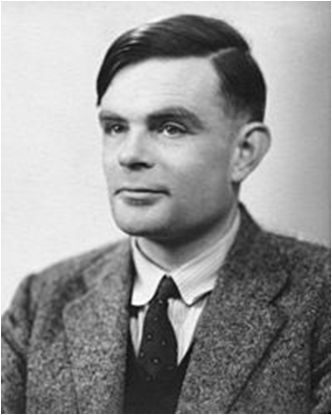
\includegraphics[height=.5\textheight]{images/turing.png}
		  		\end{center}
			\column{.6\textwidth}  		
				\begin{block}{Frase}
					\begin{center}
						{\large Machines take me by surprise with great frequency.}
					\end{center}
				\end{block}		  		
		  		\begin{block}{Quem?}
		  			\begin{center}
						{\bf Alan Turing (1912-54)} \\ Matemático, lógico, \\cientista da computação.
					\end{center}
				\end{block}
		\end{columns}
	\end{frame}
	
%------------------------------------------
\section{Revisão}	

	\begin{frame}{Exemplos}
		\begin{block}{$L(M_3)$}
		Uma máquina de Turing $M_3$ que decide $C = \{ a^i b^j c^k \mbox{ | } i \times j = k \mbox{ e } i,j,k \geq 1 \}$		
		\end{block}
	\end{frame}
	
	\begin{frame}{Exemplos}
	\begin{center}
			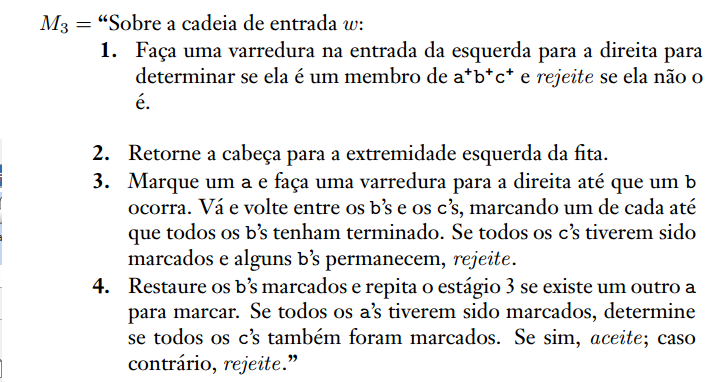
\includegraphics[height=5.5cm]{images/m3.png}
		\end{center}
	\end{frame}
	
	\begin{frame}{Exemplos}
		\begin{block}{$L(M_4)$}
		Uma máquina de Turing $M_3$ que reconhece $E = \{ \# x_1 \# x_2 \# \ldots \# x_l \mbox{ | cada } x_i \in \{ 0,1 \}^* \mbox{ e } x_i \not= x_j \mbox{ para cada } i \not= j \}$		
		\end{block}
	\end{frame}
	
	\begin{frame}{Exemplos}
	\begin{center}
			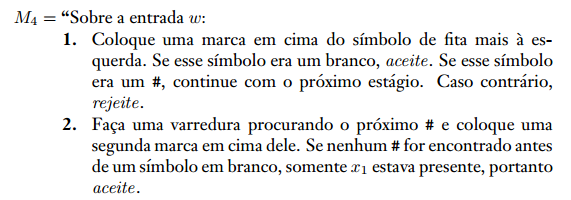
\includegraphics[height=3.5cm]{images/m4-1.png}
		\end{center}
	\end{frame}
	
	\begin{frame}{Exemplos}
	\begin{center}
			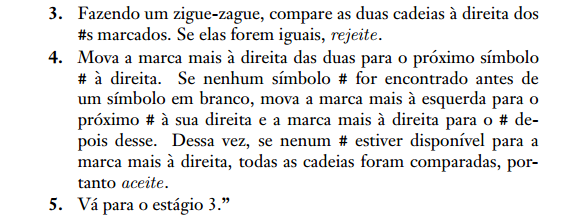
\includegraphics[height=4cm]{images/m4-2.png}
		\end{center}
	\end{frame}
    
    \subsection{MT Multifita}
	\begin{frame}[shrink]{MT Multifita}
		\begin{block}{Definição}
			Uma {\bf máquina de Turing multifita} é como uma máquina de Turing comum com várias fitas:
			\begin{itemize} 
				\item cada fita tem sua própria cabeça de leitura e escrita; 
				\item a configuração inicial consiste da cadeia de entrada aparecer sobre a fita 1, e as outras iniciar em branco;
				\item a função de transição permite ler, escrever e mover as cabeças em algumas ou em todas as fitas simultaneamente
				\begin{center}
					$\delta : Q \times \Gamma^k \rightarrow Q \times \Gamma^k \times \{E,D,P\}^k$
				\end{center}
				em que $k$ é o número de fitas.
			\end{itemize}
		\end{block}
		\begin{block}{Exemplo}
			$\delta(q_i, a_1, \ldots, a_k) = (q_j, b_1, \ldots, b_k, P, D, \ldots, E)$
		\end{block}
	\end{frame}
	
	\begin{frame}{MT Multifita}
		\begin{block}{Teorema}
			Toda máquina de Turing multifita tem uma máquina de Turing de uma única fita que lhe é equivalente.
		\end{block}
	\end{frame}
	
	\begin{frame}{MT Multifita}
		\begin{center}
			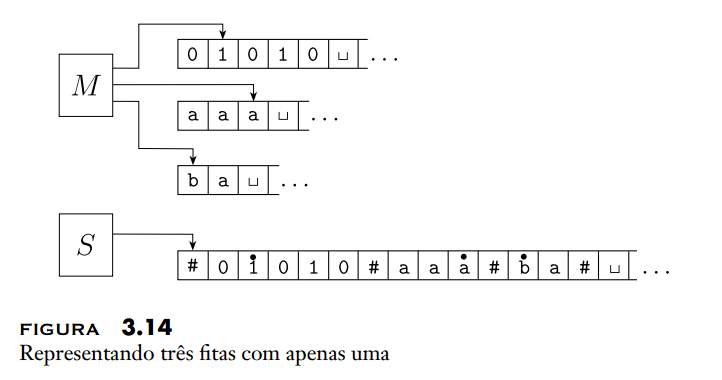
\includegraphics[height=6cm]{images/fig314.png}
		\end{center}
	\end{frame}
	
	\begin{frame}{MT Multifita}
		\begin{center}
			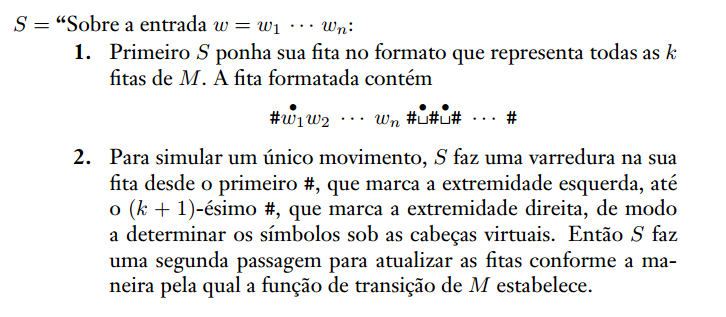
\includegraphics[height=5cm]{images/teoMt-1.png}
		\end{center}
	\end{frame}
	
	\begin{frame}{MT Multifita}
		\begin{center}
			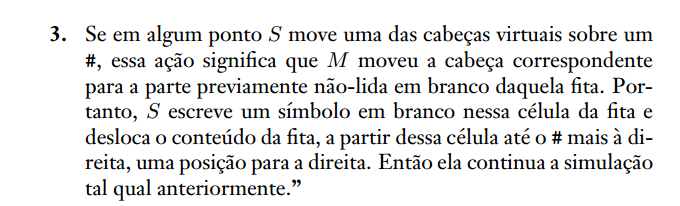
\includegraphics[height=3.3cm]{images/teoMt-2.png}
		\end{center}
	\end{frame}
	
\section{Máquina de Turing Multifita}
	
	\begin{frame}{MT Multifita}
		\begin{block}{Teorema}
			Toda máquina de Turing multifita tem uma máquina de Turing de uma única fita que lhe é equivalente.
		\end{block}
		\begin{block}{Corolário}
			Uma linguagem é Turing-reconhecível se e somente se alguma máquina de Turing multifita a reconhece.
		\end{block}
	\end{frame}
	
	\begin{frame}{MT Multifita}
		\begin{center}
			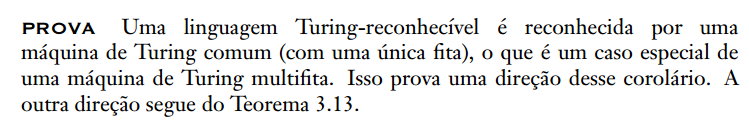
\includegraphics[height=1.8cm]{images/provaCorolario.png}
		\end{center}
	\end{frame}
	
\section{Definição de algoritmo}

	\begin{frame}{Definição de algoritmo}
		\begin{columns}
			\column{.4\textwidth}  		
		  		\begin{center}
		    		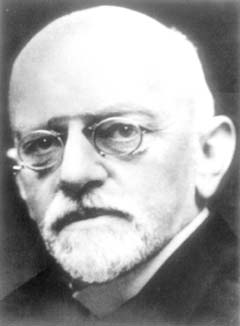
\includegraphics[height=.5\textheight]{images/hilbert.jpg}
		  		\end{center}
			\column{.6\textwidth}  		
				\begin{block}{Contribuição}
					\begin{center}
						{\large Apresentou uma noção do que seria um algoritmo no Congresso Internacional de Matemáticos em Paris, no ano de 1900.}
					\end{center}
				\end{block}		  		
		  		\begin{block}{Quem?}
		  			\begin{center}
						{\bf David Hilbert (1862-1943)} \\ Matemático alemão.
					\end{center}
				\end{block}
		\end{columns}
	\end{frame}
	
	\begin{frame}{Polinômio}
		\begin{block}{Definições}	
			Um {\bf polinômio} é uma soma de termos. Um {\bf termo} é um produto de variáveis e uma constante chamada de {\bf coeficiente}.
		\end{block}\pause
		\begin{block}{Exemplo: Termo}
			$6 \cdot x \cdot x \cdot y \cdot z \cdot z \cdot z= 6x^2 y z^3$
		\end{block}\pause
		\begin{block}{Exemplo: Polinômio}
			$6x^2 y z^3 + 3x y^2 - 10$
		\end{block}
	\end{frame}
	
	\begin{frame}{Polinômio}
		\begin{block}{Definições}	
			Uma {\bf raiz} de um polinômio é uma atribuição de valores às suas variáveis de modo que o valor do mesmo seja 0. Chamamos de {\bf raiz inteira} aquela em todos os valores atribuídos são valores inteiros.
		\end{block}\pause
		\begin{block}{Exemplo: Raiz}
			O polinômio $6x^3 y z^2 + 3x y^2 -x^3 - 10$ tem uma raiz em $x=5, y=3$ e $z=0$.
		\end{block}\pause
		\begin{block}{Exemplo: Raiz Inteira}
			A raiz do exemplo acima é uma raiz inteira.
		\end{block}
	\end{frame}
	
	\begin{frame}{Polinômio}
		\begin{block}{Problema apresentado por Hilbert}
			É possível conceber um algoritmo que teste se um polinômio tem uma raiz inteira ou não?
		\end{block} \pause
		\begin{block}{Expressão utilizada por Hilbert}
			``Um processo com o qual ela possa ser determinada por um número finito de operações''.
		\end{block} \pause
		\begin{alertblock}{Curioso}
			Não existe algoritmo que execute esta tarefa.
		\end{alertblock}
	\end{frame}
	
	\begin{frame}{Definição de algoritmo}
		\begin{columns}
			\column{.4\textwidth}  		
		  		\begin{center}
		    		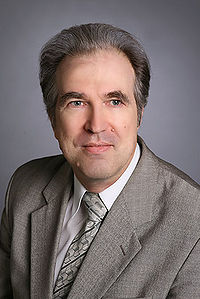
\includegraphics[height=.6\textheight]{images/yuri.jpg}
		  		\end{center}
			\column{.6\textwidth}  		
				\begin{block}{Contribuição}
					\begin{center}
						{\large Mostrou, em 1970, que não existe algoritmo para se testar se um polinômio tem raízes inteiras.}
					\end{center}
				\end{block}		  		
		  		\begin{block}{Quem?}
		  			\begin{center}
						{\bf Yuri Matijasevich (1947-)} \\ Cientista da computação e \\matemático russo.
					\end{center}
				\end{block}
		\end{columns}
	\end{frame}	
	
	\begin{frame}{Definição de Algoritmo}
		\begin{center}
    		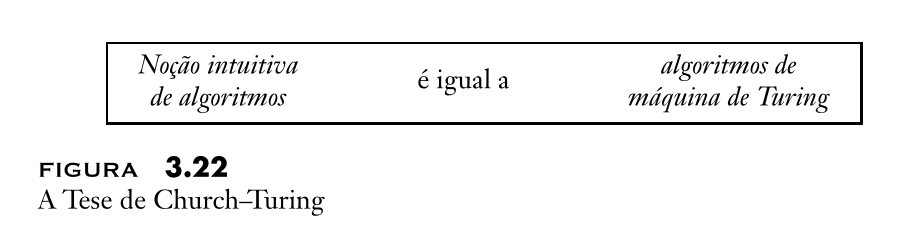
\includegraphics[width=11cm]{images/fig322.png}
  		\end{center} \pause
  		\begin{alertblock}{Conclusão}
  			Existem problemas que são algoritmicamente insolúveis.
  		\end{alertblock}
	\end{frame}
	
	\begin{frame}{Definição de Algoritmo}
		\begin{block}{Contexto}
			$D = \{ p \mbox{ | } p$ é um polinômio com uma raiz inteira$\}$
		\end{block} \pause
		\begin{block}{Problema}
			O conjunto $D$ é decidível?
		\end{block} \pause
		\begin{block}{Resposta}
			Não é decidível. Mas é Turing-reconhecível.
		\end{block}
	\end{frame}
	
	\begin{frame}{Definição de Algoritmo}
		\begin{block}{Problema análogo}
			$D_1 = \{p \mbox{ | } p$ é um polinômio sobre $x$ com uma raiz inteira$\}$
		\end{block} \pause
		\begin{block}{MT $M_1$ que reconhece $D_1$}
			$M_1$ = ``A entrada é um polinômio $p$ sobre a variável $x$.
			\begin{enumerate}
				\item Calcule o valor de $p$ com $x$ substituída sucessivamente pelos valores $0, 1,-1, 2, -2, 3, -3, \ldots$ \\Se em algum ponto o valor do polinômio resulta em $0$, {\it aceite}.
			\end{enumerate}
		\end{block}\pause
		\begin{block}{Considerações}
			$M_1$ reconhece $D_1$, mas não a decide.
		\end{block}
	\end{frame} 
	
	\begin{frame}[shrink]{Definição de Algoritmo}
		\begin{block}{Resultado obtido por Matijasevich}
			É possível construir um decisor para $D_1$. Mas não para $D$.
		\end{block} \pause
		\begin{block}{Justificativa}
			É possível obter um limitante para polinômios de uma única variável. Porém, Matijasevich provou ser impossível calcular tais limitantes para polinômios multivariáveis.
		\end{block}\pause
		\begin{block}{Limitante para polinômios de uma única variável}
			\begin{center}
				$\pm k \dfrac{c_{max}}{c_1}$
			\end{center}
			em que 
			\begin{itemize}
				\item $k$ é o número de termos do polinômio,
				\item $c_{max}$ é o coeficiente com maior valor absoluto, e
				\item $c_1$ é o coeficiente do termo de mais alta ordem.
			\end{itemize}  
		\end{block}
	\end{frame} 
	
	\section{Terminologia para descrever MTs}
	\begin{frame}{Terminologia para descrever MTs}
		\begin{block}{Níveis de descrição}
			\begin{itemize}
				\item<1,4> {\bf Descrição formal}: esmiúça todos os elementos da 7-upla, conforme definição;
				\item<2,4> {\bf Descrição de implementação}: descreve a forma pela qual a MT move a sua cabeça e a forma como ela armazena os dados na fita;
				\item<3,4> {\bf Descrição de alto nível}: neste nível não precisamos mencionar como a máquina administra a sua fita ou sua cabeça de leitura-escrita.
			\end{itemize}
		\end{block}
	\end{frame}
	
	\begin{frame}[shrink]{Exemplo}
		Seja $A$ a linguagem consistindo em todas as cadeias representando grafos não-direcionados que são conexos. Logo:
		\begin{center}
			$A = \{\langle G \rangle | G$ é um grafo não-direcionado conexo$\}$
		\end{center}\pause		
		\begin{block}{Descrição de alto nível}
			$M$ = ``Sobre a entrada $\langle G \rangle$, a codificacão de um grafo $G$:
			\begin{enumerate}
				\item Selecione o primeiro nó de $G$ e marque-o.
				\item Repita o seguinte estágio até que nenhum novo nó seja marcado:
					\begin{enumerate}
						\item Para cada nó em $G$, marque-o se ele está ligado por uma aresta a um nó que já está marcado.
					\end{enumerate}
				\item Faça uma varredura em todos os nós de $G$ para determinar se eles estão todos marcados. Se eles estão, {\it aceite}; caso contrário, {\it rejeite}''.
			\end{enumerate}
		\end{block}
	\end{frame}
	
	\begin{frame}{Exemplo}
		\begin{block}{Pergunta}
			Como seria a descrição de $M$ no nível de implementação?
		\end{block}
	\end{frame}
	
	\begin{frame}{Bônus (0,5 pt)}
		\begin{block}{Desafio}
			\begin{itemize}
				\item {\bf Problema 3.16 (a):} \\Mostre que a coleção de linguagens Turing-reconhecíveis é fechada sob a operação de concatenação.
                \item Candidaturas até amanhã (17 de maio, 09h30); 
                \item Apresentação e resposta por escrito $\rightarrow$ \\Segunda (23 de maio, 11h30); 
                \item 20 minutos de apresentação.
			\end{itemize}
		\end{block} 
        \begin{block}{Candidato}
        	???
        \end{block}
	\end{frame}
	
	\begin{frame}
		\titlepage
	\end{frame}
	
\end{document}